\begin{table}[H]
	\centering
	\captionsetup{width=0.5\textwidth}
	\caption{Resultatet från det klassiska pokertestet: Gränsvärde
	fastställt till 16.92 vid en signifikansnivå (\(\alpha\)) på
	0.05 och med 9 frihetsgrader (df). Vart ledtiden representerar
	medelvärdet för en kortleksblandning per iteration.}

	\label{tab:res-pokertest}
	\begin{subtable}[h]{0.45\textwidth}
		\centering
		\caption{\gls{gsr} Riffle Shuffle}
		\label{tab:gsr}
		\begin{tabular}{c|c|c|c}
			%\hline
			$\phantom{\bigg|}$ Iteration & $\chi^2$  & \(p\)-värde & Ledtid [ns]
			\\ \hline \hline
			3 & 233941.28 & 0 & 1681
			\\ \hline 
			4 & 7077.30 & 0 & 1687 
			\\ \hline
			5 & 449.67 & 3.38 & 1660 
			\\ \hline
			6 & 34.46 & 7.42 & 1667
			\\ \hline
			7 & 6.03 & 0.74 & 1654 
			\\ \hline
			8 & 8.50 & 0.48 & 1642 
			\\ \hline
			9 & 19.64 & 0.020 & 1582 
			\\ \hline
			10 & 8.88 & 0.45 & 1495 
			\\ \hline
			11 & 16.19 & 0.063 & 1432 
		\end{tabular}
	\end{subtable}
	\hfill
	\begin{subtable}[h]{0.45\textwidth}
		\centering
		\caption{Six Pile Shuffle}
		\label{tab:six}
		\begin{tabular}{c|c|c|c}
			$\phantom{\bigg|}$ Iteration & $\chi^2$  & \(p\)-värde & Ledtid [ns]

			\\ \hline \hline
			1 & 3854.97 & 0 & 1116 
			\\ \hline
			2 & 18.36 & 0.031 & 1124 
			\\ \hline
			3 & 12.27 & 0.20 & 1131
			\\ \hline
			4 & 5.94 & 0.75 & 1184 
			\\ \hline
			5 & 12.34 & 0.19 & 1167 
			\\ \hline
			6 & 8.89 & 0.45 & 1168 
			\\ \hline
			7 & 4.33 & 0.89 & 1211 
		\end{tabular}
	\end{subtable}

	\vspace{2em}

	\begin{subtable}[h]{0.45\textwidth}
		\centering
		\caption{\gls{soc} Pile Shuffle}
		\label{tab:soc}
		\begin{tabular}{c|c|c|c}
			$\phantom{\bigg|}$ Iteration & $\chi^2$  & \(p\)-värde & Ledtid [ns]

			\\ \hline \hline
			1 & 3349.24 & 0 & 1450 
			\\ \hline
			2 & 7.02 & 0.64 & 1465 
			\\ \hline
			3 & 19.11 & 0.024 & 1518
			\\ \hline
			4 & 7.53 & 0.58 & 1441 
			\\ \hline
			5 & 8.50 & 0.48 & 1501 
			\\ \hline
			6 & 12.34 & 0.19 & 1536 
			\\ \hline
			7 & 8.36 & 0.50 & 1577 
		\end{tabular}
	\end{subtable}
	\hfill
	\begin{subtable}[h]{0.45\textwidth}
		\centering
		\caption{Ten Pile Shuffle}
		\label{tab:ten}
		\begin{tabular}{c|c|c|c}
			$\phantom{\bigg|}$ Iteration & $\chi^2$  & \(p\)-värde & Ledtid [ns]

			\\ \hline \hline
			1 & 3349.24 & 0 & 1587 
			\\ \hline
			2 & 5.83 & 0.76 & 1654 
			\\ \hline
			3 & 4.83 & 0.85 & 1716
			\\ \hline
			4 & 5.38 & 0.80 & 1625 
			\\ \hline
			5 & 5.09 & 0.82 & 1697 
			\\ \hline
			6 & 8.80 & 0.46 & 1698 
			\\ \hline
			7 & 14.46 & 0.11 & 1710 
		\end{tabular}
	\end{subtable}
	\vspace{2em}

	\begin{subtable}[h]{0.45\textwidth}
		\centering
		\caption{Wheel Fisher-Yates Shuffle}
		\label{tab:wheel}
		\begin{tabular}{c|c|c|c}
			$\phantom{\bigg|}$ Iteration & $\chi^2$  & \(p\)-värde & Ledtid [ns]

			\\ \hline \hline
			1 & 10.71 & 0.30 & 715 
			\\ \hline
			2 & 13.46 & 0.14 & 720 
			\\ \hline
			3 & 6.66 & 0.67 & 728
			\\ \hline
			4 & 9.05 & 0.43 & 733 
			\\ \hline
			5 & 8.95 & 0.44 & 772 
			\\ \hline
			6 & 6.10 & 0.73 & 794 
			\\ \hline
			7 & 9.41 & 0.40 & 778 
		\end{tabular}
	\end{subtable}
\end{table}

\begin{figure}[H]
	\centering
	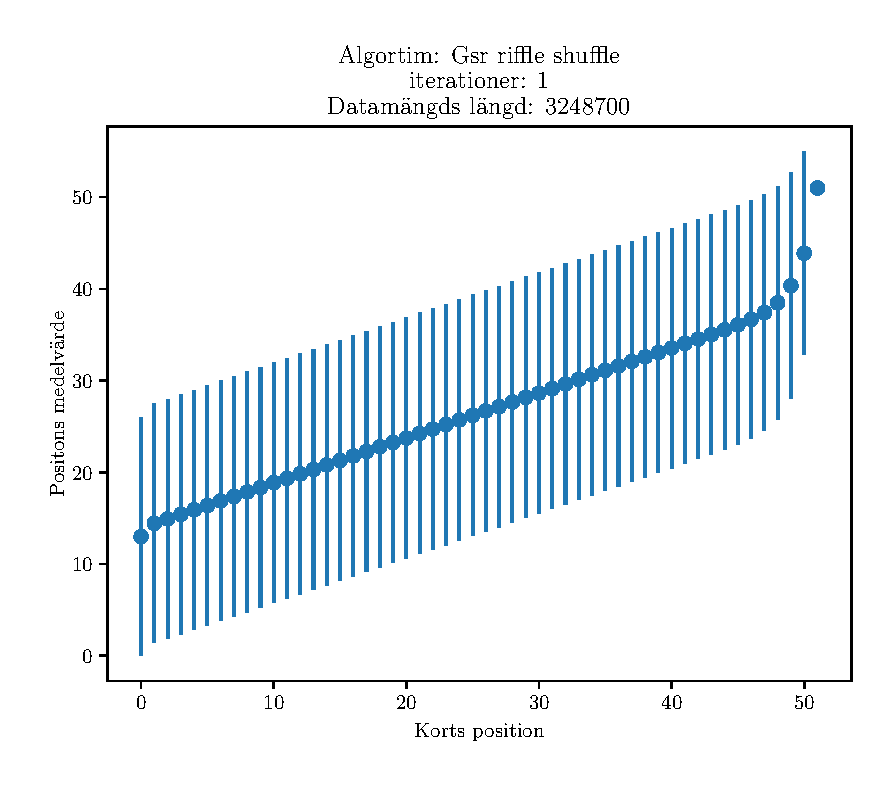
\includegraphics[width=0.8\textwidth, trim={0.8cm 0.8cm
	0.75cm 0.75cm}, clip]{gsr_riffle_shuffle-1}
	\captionsetup{width=0.5\textwidth}
	\caption{Resultatet från \gls{stdmean} testet  för \gls{gsr}
	Riffle Shuffle med \textbf{1} iteration.}
	\label{fig:gsr-1}
\end{figure}

\begin{figure}[H]
	\centering
	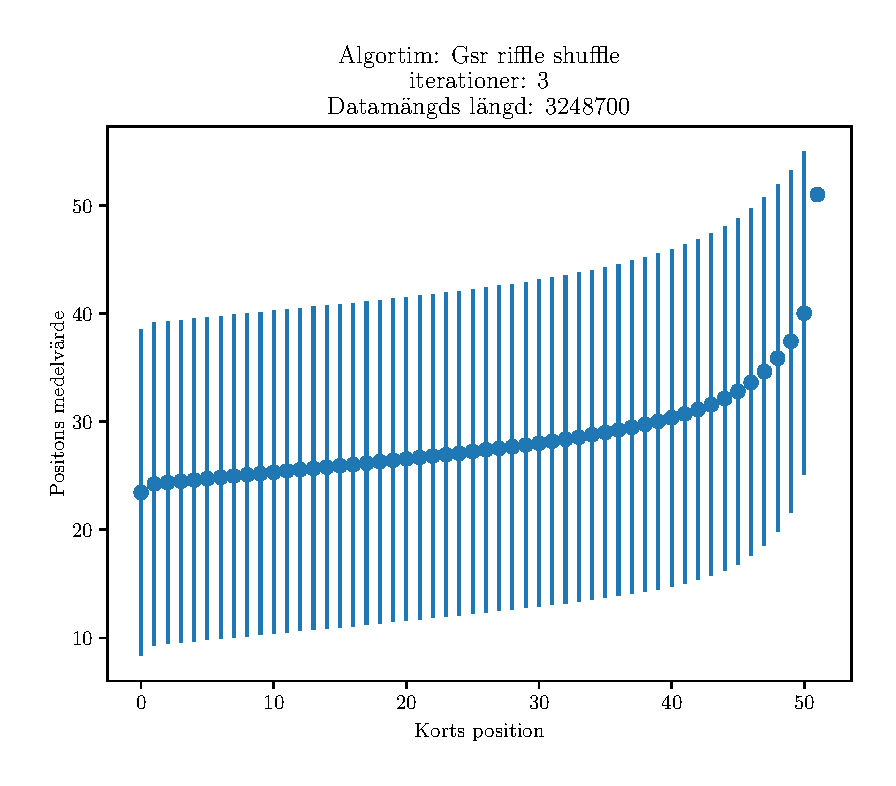
\includegraphics[width=0.8\textwidth, trim={0.8cm 0.8cm
	0.75cm 0.75cm}, clip]{gsr_riffle_shuffle-3} 
	\captionsetup{width=0.5\textwidth}
	\caption{Resultatet från \gls{stdmean} testet  för \gls{gsr}
	Riffle Shuffle med \textbf{3} iterationer.}
	\label{fig:gsr-3}
\end{figure}

\begin{figure}[H]
	\centering
	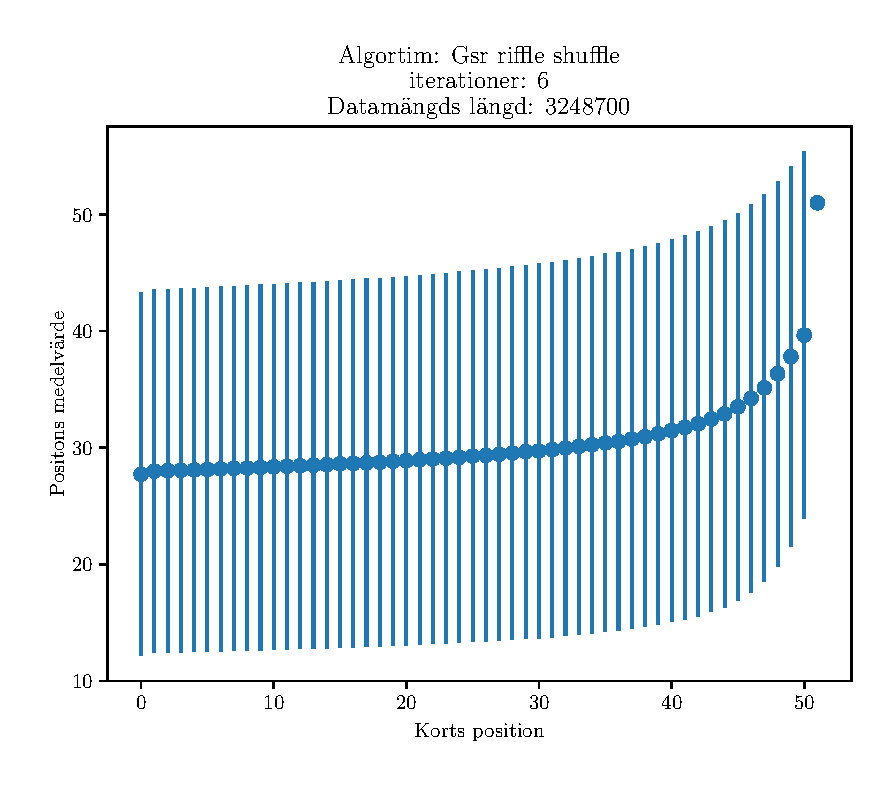
\includegraphics[width=0.8\textwidth, trim={0.8cm 0.8cm
	0.75cm 0.75cm}, clip]{gsr_riffle_shuffle-6} 
	\captionsetup{width=0.5\textwidth}
	\caption{Resultatet från \gls{stdmean} testet  för \gls{gsr} Riffle
	Shuffle med \textbf{6} iterationer.}
	\label{fig:gsr-6}
\end{figure}

\begin{figure}[H]
	\centering
	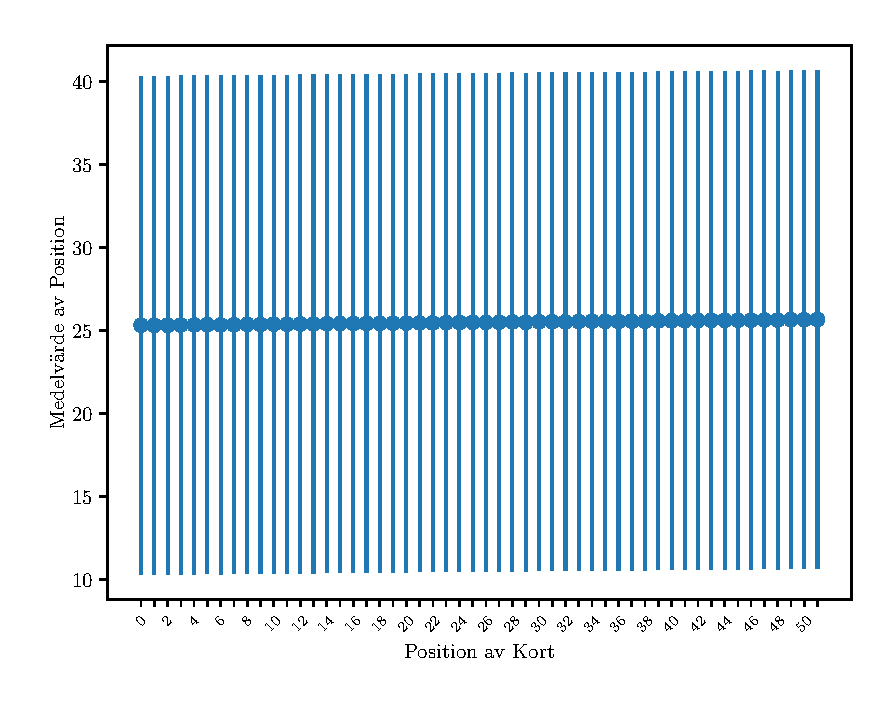
\includegraphics[width=0.8\textwidth, trim={0.8cm 0.8cm
	0.75cm 0.75cm}, clip]{gsr_riffle_shuffle-7} 
	\captionsetup{width=0.5\textwidth}
	\caption{Resultatet från \gls{stdmean} testet för \gls{gsr} Riffle Shuffle
	med \textbf{7} iterationer.}
	\label{fig:gsr-7}
\end{figure}

\begin{figure}[H]
	\centering
	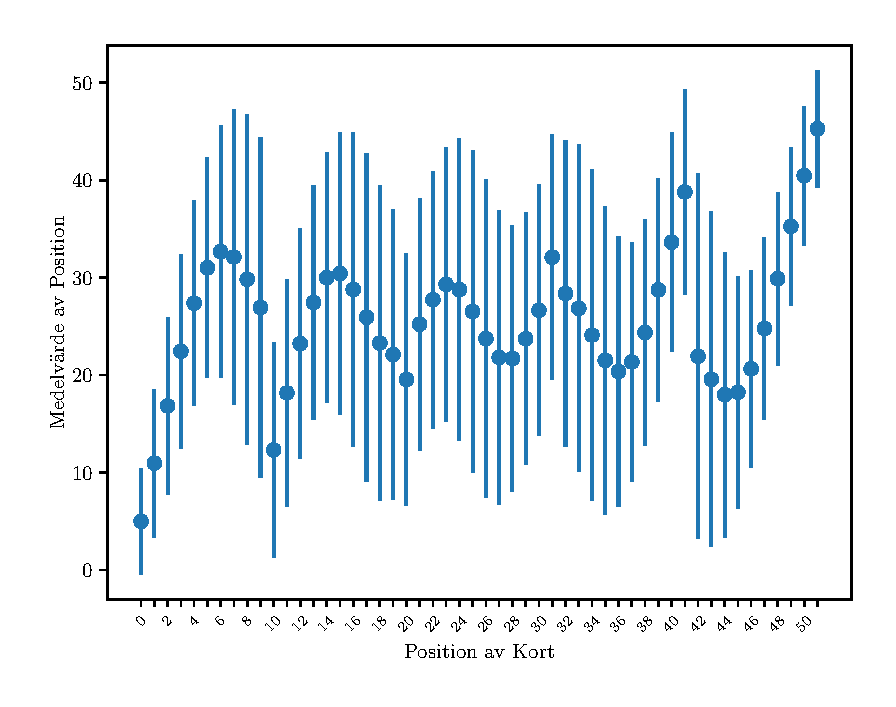
\includegraphics[width=0.8\textwidth, trim={0.8cm 0.8cm
	0.75cm 0.75cm}, clip]{six_pile_shuffle-1} 
	\captionsetup{width=0.5\textwidth}
	\caption{Resultatet från \gls{stdmean} testet för Six Pile
	Shuffle med \textbf{1} iterationer.}
	\label{fig:six-1}
\end{figure}

\begin{figure}[H]
	\centering
	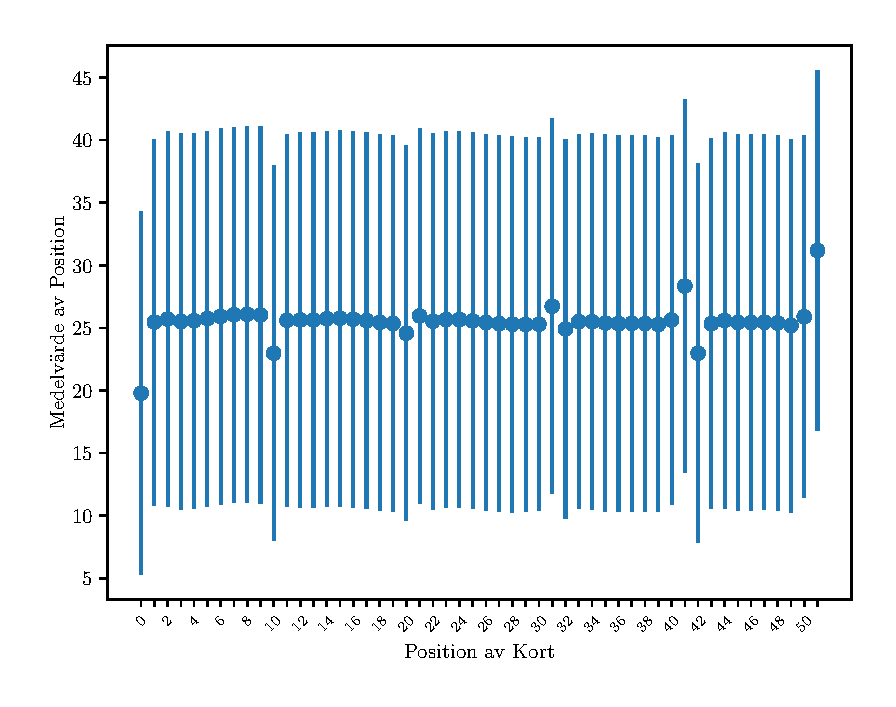
\includegraphics[width=0.8\textwidth, trim={0.8cm 0.8cm
	0.75cm 0.75cm}, clip]{six_pile_shuffle-2} 
	\captionsetup{width=0.5\textwidth}
	\caption{Resultatet från \gls{stdmean} testet för Six Pile
	Shuffle med \textbf{2} iterationer.}
	\label{fig:six-2}
\end{figure}

\begin{figure}[H]
	\centering
	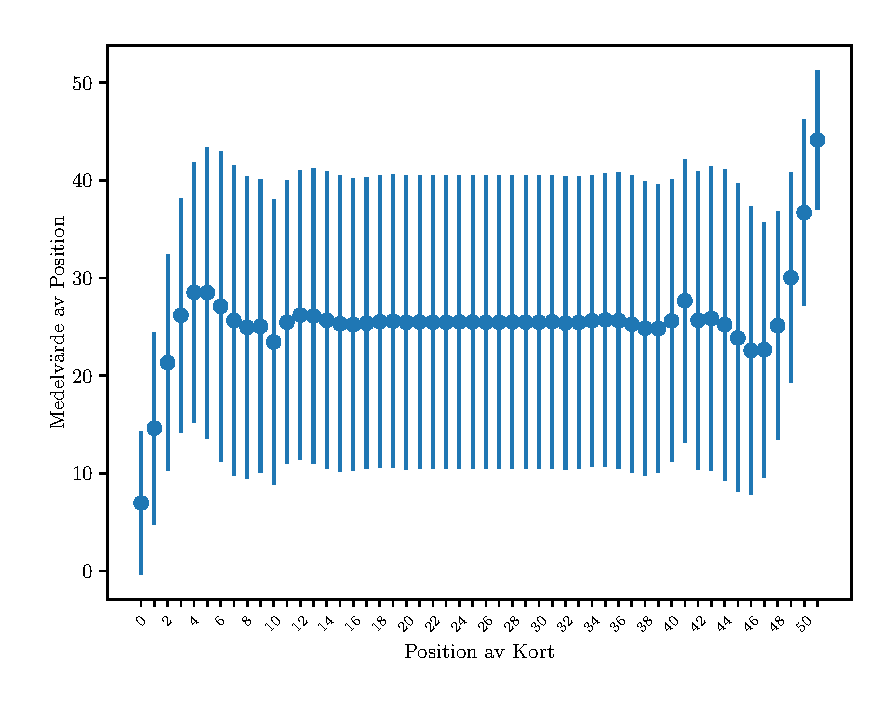
\includegraphics[width=0.8\textwidth, trim={0.8cm 0.8cm
	0.75cm 0.75cm}, clip]{soc_pile_shuffle-1} 
	\captionsetup{width=0.5\textwidth}
	\caption{Resultatet från \gls{stdmean} testet för \gls{soc} Pile
	Shuffle med \textbf{1} iteration.}
	\label{fig:soc-1}
\end{figure}

\begin{figure}[H]
	\centering
	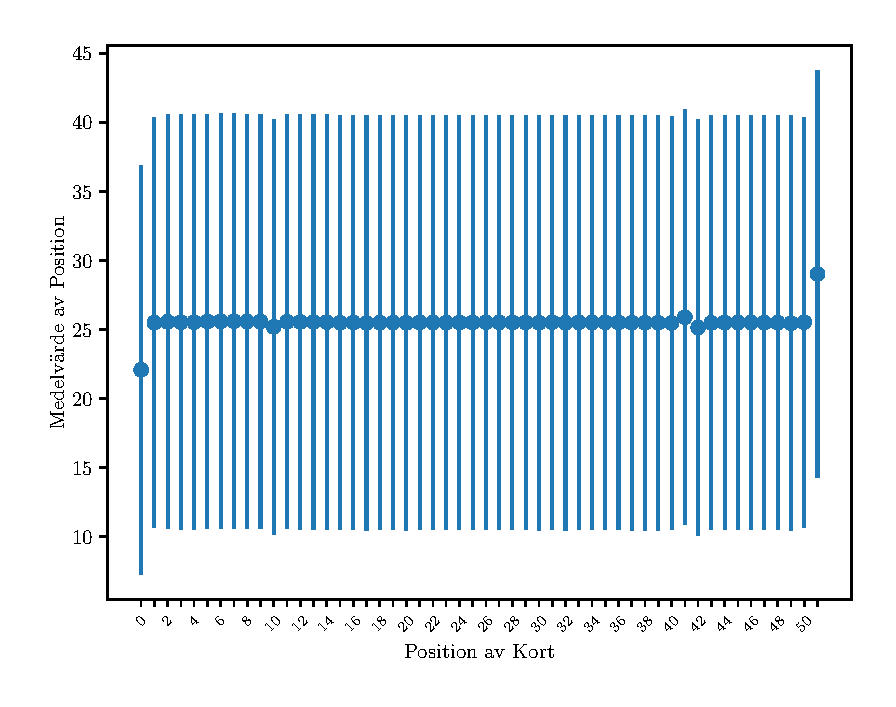
\includegraphics[width=0.8\textwidth, trim={0.8cm 0.8cm
	0.75cm 0.75cm}, clip]{soc_pile_shuffle-2} 
	\captionsetup{width=0.5\textwidth}
	\caption{Resultatet från \gls{stdmean} testet för \gls{soc} Pile
	Shuffle med \textbf{2} iterationer.}
	\label{fig:soc-2}
\end{figure}

\begin{figure}[H]
	\centering
	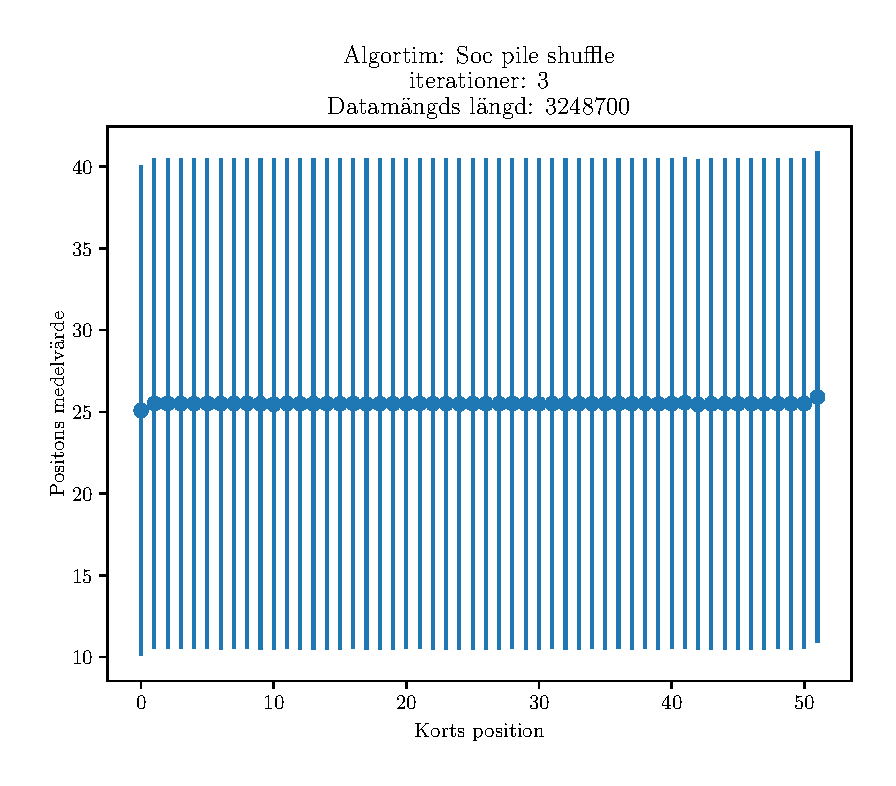
\includegraphics[width=0.8\textwidth, trim={0.8cm 0.8cm
	0.75cm 0.75cm}, clip]{soc_pile_shuffle-3} 
	\captionsetup{width=0.5\textwidth}
	\caption{Resultatet från \gls{stdmean} testet för \gls{soc} Pile
	Shuffle med \textbf{3} iterationer.}
	\label{fig:soc-3}
\end{figure}

\begin{figure}[H]
	\centering
	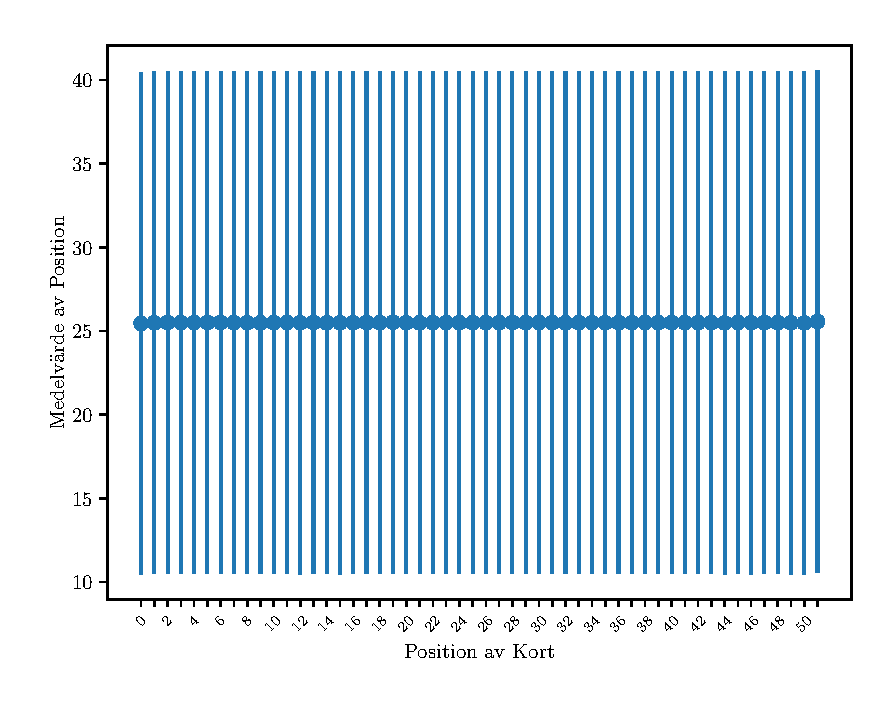
\includegraphics[width=0.8\textwidth, trim={0.8cm 0.8cm
	0.75cm 0.75cm}, clip]{soc_pile_shuffle-4} 
	\captionsetup{width=0.5\textwidth}
	\caption{Resultatet från \gls{stdmean} testet för \gls{soc} Pile
	Shuffle med \textbf{4} iterationer.}
	\label{fig:soc-4}
\end{figure}

\begin{figure}[H]
	\centering
	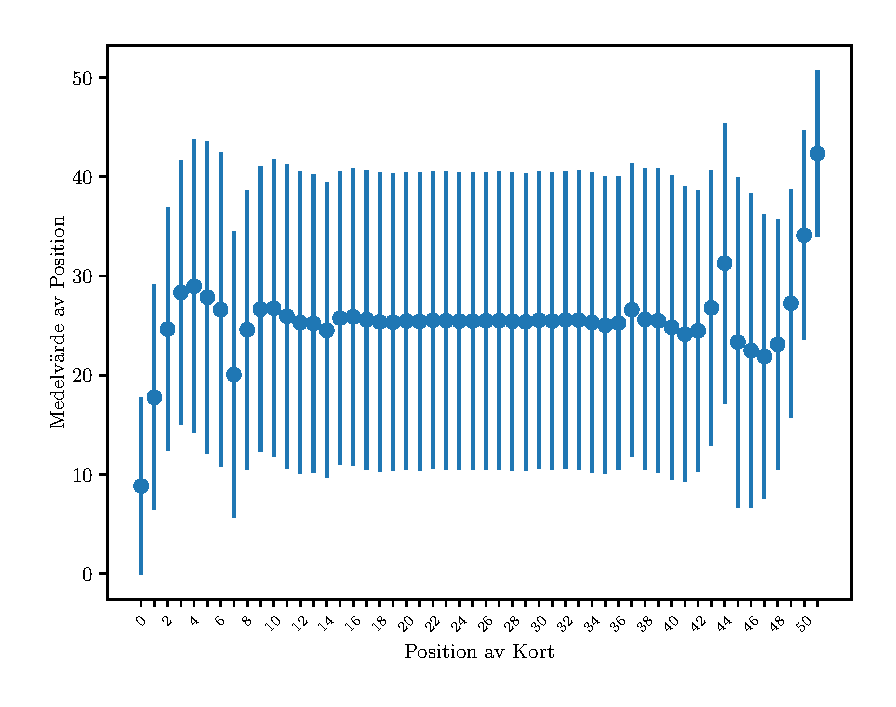
\includegraphics[width=0.8\textwidth, trim={0.8cm 0.8cm
	0.75cm 0.75cm}, clip]{ten_pile_shuffle-1} 
	\captionsetup{width=0.5\textwidth}
	\caption{Resultatet från \gls{stdmean} testet för Ten Pile
	Shuffle med \textbf{1} iteration.}
	\label{fig:ten-1}
\end{figure}

\begin{figure}[H]
	\centering
	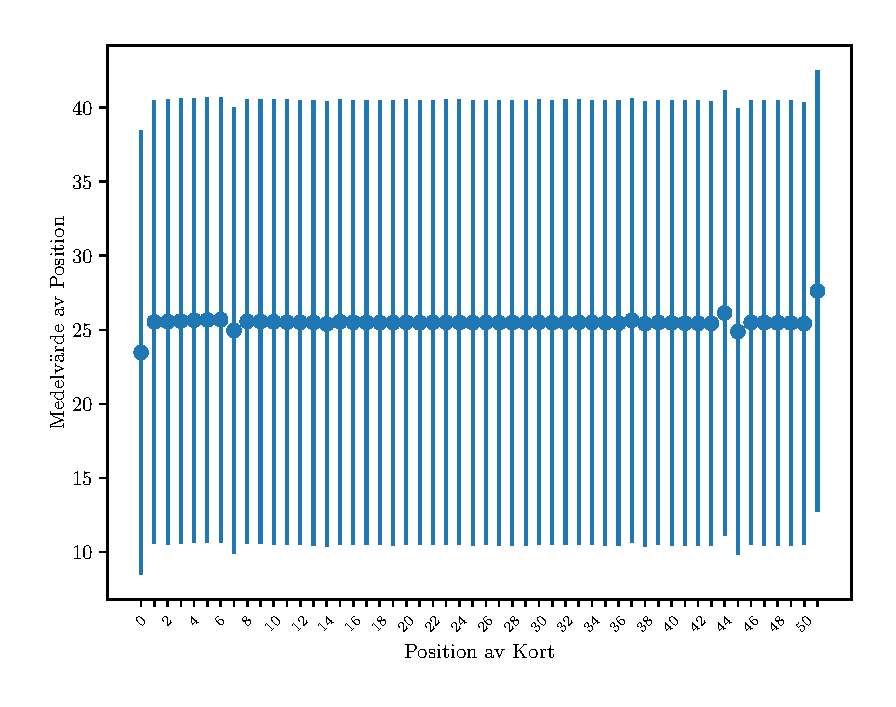
\includegraphics[width=0.8\textwidth, trim={0.8cm 0.8cm
	0.75cm 0.75cm}, clip]{ten_pile_shuffle-2} 
	\captionsetup{width=0.5\textwidth}
	\caption{Resultatet från \gls{stdmean} testet för Ten Pile
	Shuffle med \textbf{2} iterationer.}
	\label{fig:ten-2}
\end{figure}

\begin{figure}[H]
	\centering
	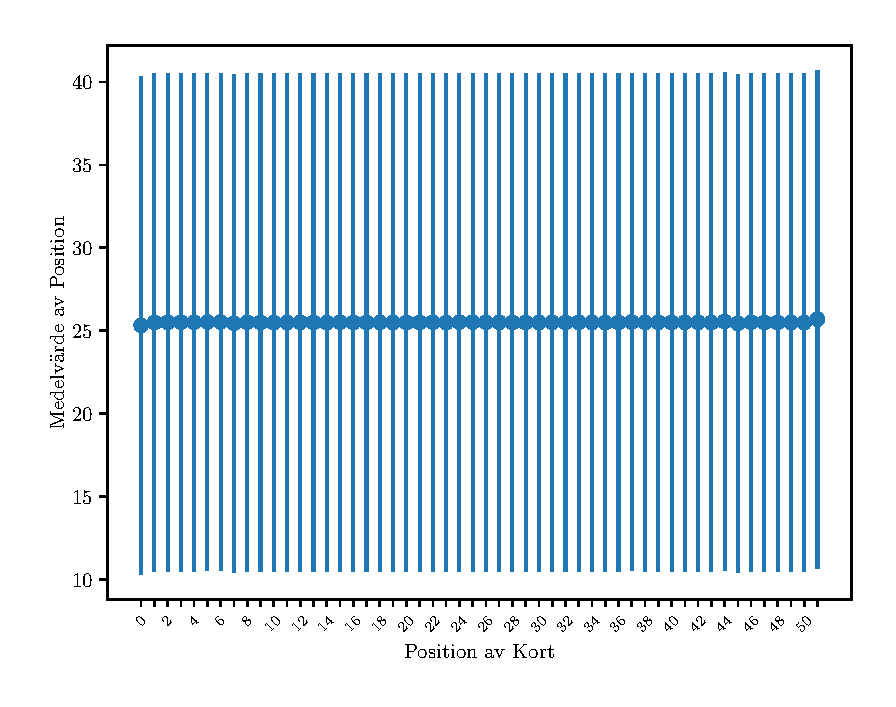
\includegraphics[width=0.8\textwidth, trim={0.8cm 0.8cm
	0.75cm 0.75cm}, clip]{ten_pile_shuffle-3} 
	\captionsetup{width=0.5\textwidth}
	\caption{Resultatet från \gls{stdmean} testet för Ten Pile
	Shuffle med \textbf{3} iterationer.}
	\label{fig:ten-3}
\end{figure}

\begin{figure}[H]
	\centering
	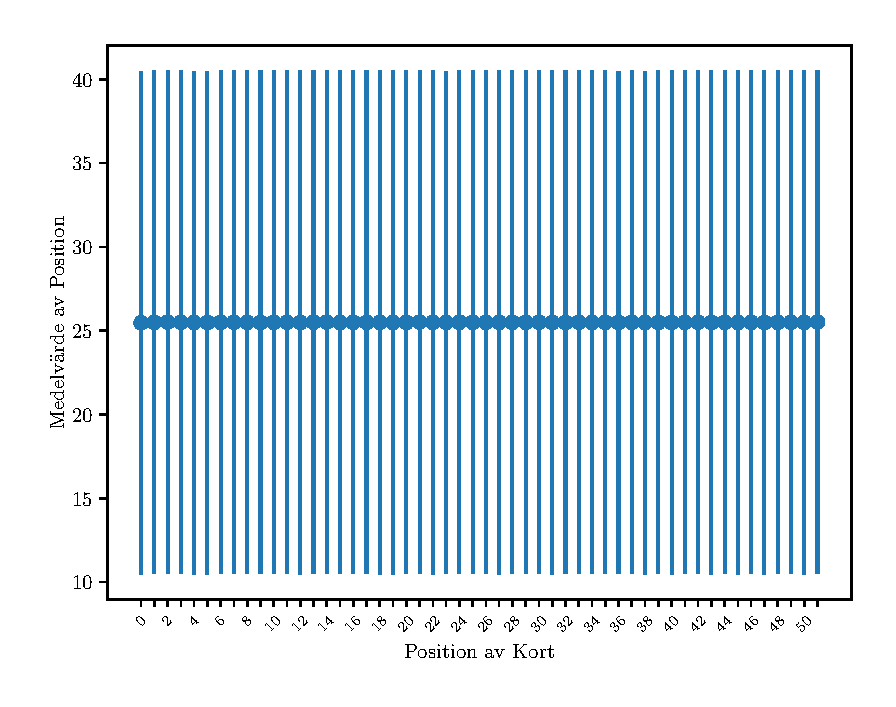
\includegraphics[width=0.8\textwidth, trim={0.8cm 0.8cm
	0.75cm 0.75cm}, clip]{ten_pile_shuffle-4} 
	\captionsetup{width=0.5\textwidth}
	\caption{Resultatet från \gls{stdmean} testet för Ten Pile
	Shuffle med \textbf{4} iterationer.}
	\label{fig:ten-4}
\end{figure}

\begin{figure}[H]
	\centering
	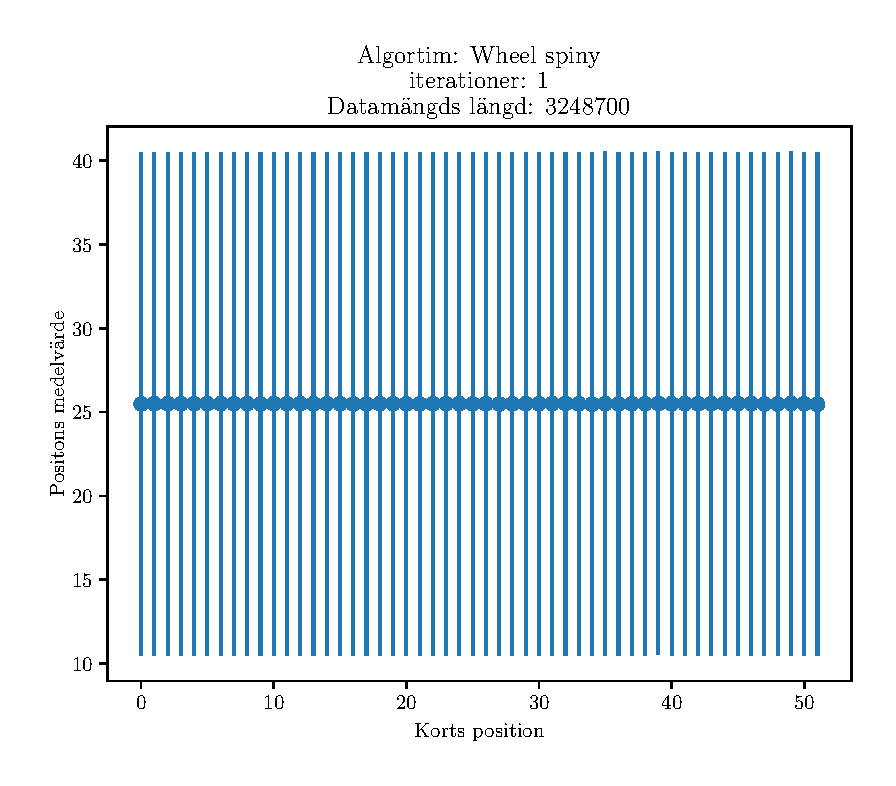
\includegraphics[width=0.8\textwidth, trim={0.8cm 0.8cm
	0.75cm 0.75cm}, clip]{wheel_spiny-1} 
	\captionsetup{width=0.5\textwidth}
	\caption{Resultatet från \gls{stdmean} testet för Wheel Fisher-Yates shuffle med \textbf{1} iteration.}
	\label{fig:wheel-1}
\end{figure}
